\documentclass{tufte-handout}

% Use this section to set the ACM copyright statement (e.g. for
% preprints).  Consult the conference website for the camera-ready
% copyright statement.



% Use this command to override the default ACM copyright statement
% (e.g. for preprints).  Consult the conference website for the
% camera-ready copyright statement.

%% HOW TO OVERRIDE THE DEFAULT COPYRIGHT STRIP --
%% Please note you need to make sure the copy for your specific
%% license is used here!
% \toappear{
% Permission to make digital or hard copies of all or part of this work
% for personal or classroom use is granted without fee provided that
% copies are not made or distributed for profit or commercial advantage
% and that copies bear this notice and the full citation on the first
% page. Copyrights for components of this work owned by others than ACM
% must be honored. Abstracting with credit is permitted. To copy
% otherwise, or republish, to post on servers or to redistribute to
% lists, requires prior specific permission and/or a fee. Request
% permissions from \href{mailto:Permissions@acm.org}{Permissions@acm.org}. \\
% \emph{CHI '16},  May 07--12, 2016, San Jose, CA, USA \\
% ACM xxx-x-xxxx-xxxx-x/xx/xx\ldots \$15.00 \\
% DOI: \url{http://dx.doi.org/xx.xxxx/xxxxxxx.xxxxxxx}
% }

% Arabic page numbers for submission.  Remove this line to eliminate
% page numbers for the camera ready copy
% \pagenumbering{arabic}

% Load basic packages
\usepackage{balance}       % to better equalize the last page
\usepackage{graphics}      % for EPS, load graphicx instead 
\usepackage[T1]{fontenc}   % for umlauts and other diaeresis
\usepackage{txfonts}
\usepackage{mathptmx}
\usepackage[pdflang={en-US},pdftex]{hyperref}
\usepackage{gensymb}
\usepackage{booktabs}
\usepackage{textcomp}
\usepackage[inline]{enumitem}
\usepackage{subcaption}

% Some optional stuff you might like/need.
\usepackage{microtype}        % Improved Tracking and Kerning
% \usepackage[all]{hypcap}    % Fixes bug in hyperref caption linking
\usepackage{ccicons}          % Cite your images correctly!
% \usepackage[utf8]{inputenc} % for a UTF8 editor only

% If you want to use todo notes, marginpars etc. during creation of
% your draft document, you have to enable the "chi_draft" option for
% the document class. To do this, change the very first line to:
% "\documentclass[chi_draft]{sigchi}". You can then place todo notes
% by using the "\todo{...}"  command. Make sure to disable the draft
% option again before submitting your final document.
\usepackage{todonotes}
\usepackage{soul}

% Paper metadata (use plain text, for PDF inclusion and later
% re-using, if desired).  Use \emtpyauthor when submitting for review
% so you remain anonymous.
\def\plaintitle{Interacting with Smart Consumer Cameras: Exploring
  Gesture, Voice, and AI Control of Video Streaming}
\def\plainauthor{First Author, Second Author, Third Author}

\def\emptyauthor{}

\def\plainkeywords{video; cameras; video conference; livestreaming;
  personal devices; gesture; voice control; AI\@; UI\@; wizard of oz;
  elicitation study. }

\def\plaingeneralterms{Human Factors}

% llt: Define a global style for URLs, rather that the default one
\makeatletter
\def\url@leostyle{%
  \@ifundefined{selectfont}{
    \def\UrlFont{\sf}
  }{
    \def\UrlFont{\small\bf\ttfamily}
  }}
\makeatother
\urlstyle{leo}

% To make various LaTeX processors do the right thing with page size.
\def\pprw{8.5in}
\def\pprh{11in}
\special{papersize=\pprw,\pprh}
\setlength{\paperwidth}{\pprw}
\setlength{\paperheight}{\pprh}
\setlength{\pdfpagewidth}{\pprw}
\setlength{\pdfpageheight}{\pprh}

% Make sure hyperref comes last of your loaded packages, to give it a
% fighting chance of not being over-written, since its job is to
% redefine many LaTeX commands.
\definecolor{linkColor}{RGB}{6,125,233}
\hypersetup{%
  pdftitle={\plaintitle},
% Use \plainauthor for final version.
%  pdfauthor={\plainauthor},
  pdfauthor={\emptyauthor},
  pdfkeywords={\plainkeywords},
  pdfdisplaydoctitle=true, % For Accessibility
  bookmarksnumbered,
  pdfstartview={FitH},
  colorlinks,
  citecolor=black,
  filecolor=black,
  linkcolor=black,
  urlcolor=linkColor,
  breaklinks=true,
  hypertexnames=false
}

% create a shortcut to typeset table headings
% \newcommand\tabhead[1]{\small\textbf{#1}}

% End of preamble. Here it comes the document.
\begin{document}

\title{\plaintitle}

\numberofauthors{3}
\author{%
  \alignauthor{Leave Authors Anonymous\\
    \affaddr{for Submission}\\
    \affaddr{City, Country}\\
    \email{e-mail address}}\\
  \alignauthor{Leave Authors Anonymous\\
    \affaddr{for Submission}\\
    \affaddr{City, Country}\\
    \email{e-mail address}}\\
  \alignauthor{Leave Authors Anonymous\\
    \affaddr{for Submission}\\
    \affaddr{City, Country}\\
    \email{e-mail address}}\\
}

\maketitle

\begin{abstract}
  Livestreaming and video calls have grown in popularity due to the
  increased connectivity and advancements in mobile devices. Our
  interactions with these cameras are limited as the cameras are
  either fixed or manually remote controlled.  Here we present a
  Wizard-of-Oz elicitation study to inform the design of interactions
  with smart 360\textdegree\ cameras or robotic mobile desk cameras
  for use in video-conferences and live-streaming situations.  Our
  results show participants starting with Cartesian directions (``move
  90\textdegree\ left'') but move slowly to object based commands
  (``show the whiteboard''). There was an overall preference for
  devices, like static cameras or automatic AI camera robots, that can
  minimize distraction. We also find preferences for devices that can
  show they demonstrate an understanding of video-meeting context:
  These devices create the feeling of connection to the remote
  participant.  Finally, we detail interaction techniques and design
  insights to inform the next generation of personal video cameras for
  streaming and collaboration.
\end{abstract}

\category{H.4.3.}{Communications Applications}{Computer
conferencing, teleconferencing, and videoconferencing}
\category{H.5.m.}{Information Interfaces and Presentation
  (e.g. HCI)}{Miscellaneous} 

\keywords{\plainkeywords}

\section{Introduction}
Personal media streaming has entered a new
age~\cite{Lottridge:2017:TLT:3098279.3098540} with the growth of
Internet-enabled cameras and smartphones coupled with various
streaming services and video calling applications. While in the past
video-streaming was found in enterprise conference calls, it now also
enables self-run Internet ``TV'' shows on YouTube, social media
livestreams on Facebook, and personal broadcasts on Twitch.  In many
of these cases, people resort to holding a cameraphone, using a laptop
screen mounted webcam, or even having installed setups with green
screens, lighting, and picture in picture broadcasts.

Consider the solo broadcaster or set of broadcasters trying to queue
various cameras. Typically they would rely on a display camera zoomed
into a fixed area so they could show a item and then have a second
camera to capture themselves or the room.  Cameras could be triggered
via keyboard press. If they had one articulating camera, it could be
driven via remote control.  Both cases require various levels of
interaction from the broadcaster.  

Currently, we are faced with two recent advancements.  First, cameras
now have high resolution captures well beyond 1080p HD\@. Many
consumer cameras shoot video in 4k or 6k and can capture wide or
360\textdegree\ fields of view, allowing one to crop out an HD
frame. Second, artificial intelligence (AI) technologies have vastly
improved in the areas of object detection, face identification, and
voice recognition.  Towards this, we ask how would one control such a
high-resolution AI-enabled personal camera.

In this article, we present a Wizard-of-Oz elicitation study to
understand how people would interact with a smart personal camera that
could either (1) pick the person or objects to focus on automatically,
(2) could be controlled by visual hand gestures like pointing, or (3)
could be voice controlled to focus on a person or object.  In the
study, we not only surface what kind of visual or audio commands one
would use to control such a personal video camera, but also how
different cameras' interaction techniques can lead to the camera
becoming a participant in the meeting and can facilitate deeper
connections with remote participants.  Finally, we illustrate how this
research can inform the design of future enterprise or personal video
cameras for meetings or livestreaming.

\section{Related Work}
The broader research work in video conferencing, chat rooms, and
livestreams is expansive.  Telepresence systems have tried to connect
people through extensive camera augmentation and
registration~\cite{Dunnigan:2015:ETT:2733373.2807400} as well as
simpler side-by-side~\cite{Tanner:2010:IRC:1753846.1754007}
arrangements.  Beyond work contexts, livestreaming on the Internet has
grown~\cite{Lottridge:2017:TLT:3098279.3098540} due to expanding
connectivity and network-enabled cameras (and cameraphones). In this
article, we focus less on improving image
fidelity~\cite{Wang:2016:APL:2987443.2987453} and/or the mechanics of
building an AI system for object recognition. Instead we focus on
experiences, people, and behaviors.

\subsection{Consumer Devices}
There has been some growth recently in video cameras for meetings,
mostly in the enterprise sector. New devices like the Meeting
Owl\footnote{\url{https://www.owllabs.com/}} and Sony Xperia
Hello!\footnote{\url{http://www.sony.jp/xperia-smart-products/products/G1209/}}
provide tower-like single lens 360\textdegree\ cameras for video
calling.  The Meeting Owl has a top facing camera and is designed for
boardroom use.  The Xperia Hello! has a front skewed single lens
camera for meetings or personal calling. Other devices, like the
Amazon Echo Show and Spot, have a similar camera to that on a laptop
of tablet device. Finally, the Google Snap camera is a device designed
to be placed in vantage points where one might need photos or video
marketed for non-enterprise environments.

\subsection{User Behaviors in Live Streams \& Video Conferences}
One common scenario for live streaming includes a conversation between
individuals or a group of people who are sitting in a room or fixed
location. However, as streaming becomes easier and more mobile, people
may wish to view multiple streams from different perspectives, such as
at a large public event~\cite{hamilton2016rivulet}.  Audience members
may also interact with streamers in other ways such as through chat or
voting mechanisms to influence what
happens~\cite{lessel2017let}. However, enabling presenters to easily
share their perspectives and activities with viewers continues to be
an important area of focus as well.

One issue that has emerged in single, or fixed-camera video streaming
settings has to do with how people go beyond being ``talking heads''
to showing physical items or highlighting movements, as in a
performance~\cite{reeves2015d}. A study of how people share physical
artifacts (whiteboards, notebooks, mobile phone screens) with remote
meeting participants over video conferencing revealed that this
behavior is difficult and can be disruptive to the flow of the
meeting~\cite{Marlow:2016:BTH:2818048.2819958}.

Other work~\cite{ursu2015experimental} has looked at how multiple
fixed cameras might be used to automatically switch between different
views of people engaging in a distributed task. Initial explorations
in this space suggest that automatically switching camera viewpoints
could be a scalable solution when people are distributed across
multiple sites; however, such a setup still requires that rooms be
outfitted with several pieces of hardware that are not easily
portable.

\subsection{Automatic Camera Operators}
Another area of research is on the automatic camera operator. This
includes proposing a set of rules for an automatic
camera-person~\cite{Strubbe:2001:UVC:634067.634264} to learning where
to focus a pan/tilt/zoom (PTZ) camera based on previous user
interactions~\cite{liu2003learning} to automatic positioning of
multiple PTZ cameras to maximize the captured video information for
passive viewers---providing the best close-up view with limited
cameras~\cite{liu2005online}.  Typically, when multiple cameras are in
operation, camera selection is done via algorithm, such as a
constraint satisfaction
problem~\cite{Janzen:2008:CSU:1496984.1497038}, or done via community
cooperation~\cite{Sa:2014:LMC:2584567.2584573}.  More sophisticated
controls create camera-sensing
networks~\cite{Qureshi:2010:CSV:1865987.1866017} or use a set of
distributed smart cameras and with gesture
sensing~\cite{Lin:2010:SSA:1721695.1721704} to control the queuing.

\subsection{Interactions}
Hand gestures have been a common interaction technique for video and
for remote control~\cite{Dezfuli:2012:PIP:2325616.2325623}.  This is
of particular interest given the current advancements in AI and the
availability of large scale, crowdsourced datasets for gesture
recognition such as the 20BN-Jester Dataset V1\footnote{The
  20BN-JESTER Dataset \ccbyncnd\ is a large collection of
  densely-labeled video clips that show humans performing pre-defined
  hand gestures in front of a laptop camera or webcam. The dataset was
  created by a large number of crowd workers. It allows for training
  robust machine learning models to recognize human hand
  gestures. \url{https://twentybn.com/datasets/jester}}. One question
we wish to investigate is how people would interact through gestures
for a personal desk robot.  Bearing the most similarity to our work is
the recent Wizard-of-Oz Human-Drone
Interaction~\cite{Cauchard:2015:DME:2750858.2805823} experiment. While
hand gestures have been explored before for remote controlling
quadcopter drones~\cite{Stoica:2014:RCQ:2559636.2559853}, Cauchard et
al.'s elicitation study showed how people would control a personal
quadcopter through gesture and voice.

Also similar to our work is a recent observational lab study in
which participants critiqued pairs of physical prototypes (prosthetic
hands) for a face-to-face or remote
collaborator.~\cite{Mok:2017:CPP:3064663.3064722}. Here, details in
physical prototypes were shared in two different contexts. The authors
found that traditional media sharing experiences are optimized for an
upwards gaze whereas tabletops focus downward; they suggest
head-mounted displays to keep media spaces in peripheral vision while
downward attention is focused on an artifact or object.  They also
suggest prioritizing the camera preview window as theirs was
rendered too small in their experiment.

\begin{figure}
  \centering
  \includegraphics[angle=180,width=\columnwidth]{figures/ricoh-cozmo}
  \caption{\label{fig:cameras} The Ricoh Theta V, a 4k 360\textdegree\ camera,
    (left) and the Anki Cozmo robot (right).}
\end{figure}

\section{Method \& Experiment}
We present a Wizard-of-Oz elicitation study to understand the kind of
interactions people would have with smart video cameras in a
livestream or video-conference context.  We used an office space with
a table and a whiteboard and a set of printed material to simulate a
conversation across two locations where two collocated participants
shared materials and information with a remote attendee using four
different camera setups and interaction modalities:
\begin{enumerate}
\item\label{item:1} A stationary 4k 360\textdegree\ camera that
  automatically identifies the salient person or object and streams
  it.
\item\label{item:2} A small moving camera-robot that pans on the
  table to automatically identify the salient person or object and
  streams it.
\item\label{item:3} A small moving camera-robot that pans on the
  table and responds to visual gestures to turn to the salient person
  or object and stream it.
\item\label{item:4} A small moving camera-robot that pans on the
  table and responds to voice commands to turn to the salient person
  or object and stream it.
\end{enumerate}
The 4k 360\textdegree\ camera was a Ricoh Theta V and the small moving
camera-robot was an Anki Cozmo (see Figure~\ref{fig:cameras}).  Both
cameras are consumer-level devices retailing for \$400 and \$180
respectively.  An experimenter remote controlling the Cozmo over WiFi
was in an adjacent office with a confederate who was connected to the
participants via a speakerphone to ask questions and comment.  This
setup mirrors a remote participant on a video call with no camera of
their own (thus not drawing eye contact from the participants) which
is also analogous to a typical livestream.  The difference between the
two scenarios is that the confederate can give audio feedback whereas
a livestream would rely on text comments as feedback.

For each case, minimal instruction was given to the participants. For
each condition this was:
\begin{itemize}
\item Condition~\ref{item:1}: ``The camera will use
  AI to automatically find and stream people and objects in the room
  relevant to the conversation.''
\item Condition~\ref{item:2}: Same as Condition~\ref{item:1}.
\item Condition~\ref{item:3}: ``The robot-camera will respond to hand
  gestures to move.''
\item Condition~\ref{item:4}: ``The robot-camera will respond to voice
  commands if you first address it as `hey robot'.''  This condition
  mimics modern voice appliances such as Amazon Alexa, Apple Siri.
\end{itemize}
We did not refer to either camera by brand or name to avoid
anthropomorphism of the Cozmo robot and while the Cozmo has various
expressive face/eye animations, we kept its expression in a neutral
repose.

\subsection{Participants}
For this study, we recruited 10 volunteers (2 females, 8 males) from
our institution.  All of the participants were college educated and
were somewhat familiar with 360\textdegree\ or robot-articulating
cameras.  Additionally, all of the participants reported they
generally felt comfortable around cameras in the room.  There was also
an even distribution of participants who said they were easily
distracted or not easily distracted.

\subsection{Task}
The basic task among each participant pair was to discuss various
electronics or accessories to purchase for a company.  We separated
this into four tasks, one per category type:
\begin{enumerate*}[label=(\alph*)]
\item laptop,
\item tablet,
\item phone, and
\item backpack/messenger bag
\end{enumerate*}. Two items from each task type were selected and
printed out as technical specifications and prices from their
associated web pages.  The whiteboard contained a handwritten (but
incomplete) table of regions, employee ranks, and budget prices.
Conditions and tasks were matched randomly and counterbalanced for
each pair (four in total). Each participant had one item assigned to
them to explain and share with the remote participant.  For example,
for Condition~\ref{item:3} and task \textit{phone}, one participant
received printouts for an iPhone X and the other received printouts
for a Google Pixel 2.  Both participants were asked to discuss each
device as it relates to a price point, region, or employee rank on the
white board.  The camera-robot was the only broadcasting feed and
responded to visual gestures (Condition~\ref{item:3}) to move.


\begin{figure}
  \centering
  \includegraphics[width=\columnwidth]{figures/insert-page}
  \caption{\label{fig:insertpage} Here the robot camera has been
    directed via gesture to look at the whiteboard.  A participant
    (P2) wanted to show a handout which he just put in the camera's
    field of vision instead of directing the robot camera back to
    him.}
\end{figure}

\subsection{Procedure}
An office equipped with a table, chairs, and a whiteboard was
outfitted with several printouts. A small (GoPro) camera was mounted
to the far corner of the whiteboard, opposite side of the experiment
related whiteboard content, to record the experiment and participants
were instructed to ignore it.  Participants were first given 5 minutes
to review all the printouts. Conditions and tasks were randomly
assigned then, before each condition, an experimenter brought a camera
device into the room, briefly explained its capabilities and discussed
the task. The participants were told that an executive from corporate
headquarters (the confederate) was connected via speakerphone.

The experimenter then left and the confederate prompted the session to
begin.  The confederate minimally prompted for information or visuals
about the whiteboard and printouts if these were not spontaneously
provided by the participants. As the Cozmo's resolution is rather low,
the confederate had a copy of all the handouts but did not disclose
this to the participants. This allowed the confederate to ``play
along'' and overcome the current limitations with the camera-robot.
Figure~\ref{fig:insertpage} shows an example of the camera's fidelity.

Upon completion of the condition-task pair, the experimenter returned,
collected the device and handed the participants a short survey to
fill out.  Once completed, the surveys were collected, a device was
returned to the room and the next condition-task pair started.  There
were four condition-task pairs in total and the full experimental
session lasted around 30 minutes overall. At the end of the last
condition-task pair, a final survey was completed by the participants,
and they participated in a short interview/discussion with the two
experimenters in order to collect additional comments about their
reactions to the different conditions.

\subsection{Surveys and Exit Interview}
After each condition-task pair, participants were handed a short
survey.  After the final pair, they were handed an additional overall
survey. Once completed, the experimenters asked the participants if
there was any additional feedback, comments, or questions. Each of the
condition-task surveys asked questions (on a 5 point Likert scale from
strongly disagree to strongly agree) related to the camera condition:
was the camera useful, did they know what the camera was looking at
during the meeting, did they want to control the camera/did they feel
they could control the camera. Additionally, there were two open-ended
questions asking participants what they liked and disliked about the
technology they used in that condition.

The final survey gathered demographics (age, gender, education),
experience with robotic or 360\textdegree\ cameras, how comfortable
they are with being recorded, if the camera was distracting, and
a self-reported assessment of whether they were easily distracted in
general. We also asked if they wanted to be able to toggle the
camera's recording state, and we asked them to rank the four
conditions in order of preference.  Finally we asked if there was any
other way they would have liked to control the camera and if there was
anything else aside from people, papers, and whiteboards that they
would want the camera to know about. 

\begin{figure*}
  \centering
  \begin{subfigure}[b]{0.6\textwidth}
  \includegraphics[width=\textwidth]{figures/likerts/likert-woz-1}
  \caption{\label{fig:likert-overview} Across all four conditions, how
  useful and understandable was each camera.}
\vspace{1pc}  
\end{subfigure}
\begin{subfigure}[b]{0.6\textwidth}
  \centering
  \includegraphics[width=\textwidth]{figures/likerts/likert-woz-2}
  \caption{\label{fig:likert-no-control} For the \textit{fully AI}
    conditions, how much did participants want to control the camera.}
\vspace{1pc}
\end{subfigure}
\begin{subfigure}[b]{0.6\textwidth}
  \centering
  \includegraphics[width=\textwidth]{figures/likerts/likert-woz-3}
  \caption{\label{fig:likert-control} For the controllable cameras,
    how easy it was to control the camera and how distracting were the
  cameras.}
\vspace{1pc}
\end{subfigure}
  \caption{\label{fig:likerts} Answers to the Likert survey
    questions. Voice control was the most useful but not the first
    preference; participants often wanted a view screen for each
    camera, but found the 360\textdegree\ camera the most unknown to
    what it was doing (Figure~\ref{fig:likert-overview}).}
\end{figure*}

\section{Results}
When asked to rate the four conditions in order of preference, the
360\textdegree\ degree camera was the favorite of 5/10
participants. The next most favored condition was the AI robot (3/10
participants), followed by voice control (2/10 participants).  The
gesture control condition was selected as the second favorite option
by 4 out of 10 participants.  Figure~\ref{fig:likerts} presents the
distribution of responses to the survey questions relating to the
usefulness, awareness of, degree of control over, and distraction
caused by the different conditions.

To further unpack the variation in preferences between the different
interaction methods, we now discuss behaviors observed during the
experiment as well as open-ended comments provided by participants for
the four different conditions. These provide some insights into the
ways in which the different technological affordances of the
360\textdegree\ and robot cameras influenced the behaviors and
attitudes of participants with regards to sharing their environments
with the meeting viewer.

\subsection{360\textdegree}
During the 360\textdegree\ session, most participants were fairly
comfortable with the technology even though not all of them had used
such a device before.  For this condition, 3 participants selected
``Strongly Agree'' with the statement that the camera was useful, 5
selected ``Agree'' and 2 were neutral. However, the 360-degree camera
was rated significantly lower than the three robotic conditions in
terms of agreement with the question ``I knew what the camera was
looking at.''  Participants brought up the point that the
360\textdegree\ camera required the least amount of input or
interaction from the two presenters in the room (because the remote
person could see everything and control what they focused on). The
benefit of this setup was that it gave greater agency to the remote
viewer:
\begin{quote}
  ``The camera was for you [the remote participant], not for me and I
  wanted you to be in charge of what you were looking at, it's not my
  job.'' (P6)
\end{quote}However, while this benefited the remote participant, the
two co-located meeting participants lacked awareness of the remote
party's focus. This was sometimes challenging because
\begin{quote}
  ``it's always visible and the remote user can watch me\ldots though I
  feel being monitored I also wonder whether the remote users have
  time and effort to monitor all the stuff in the 360 camera'' (P9)
\end{quote}

\begin{figure}
  \centering
  \begin{subfigure}[b]{0.85\columnwidth}
    \centering
  \includegraphics[trim={0 30cm 0
    15cm},clip,width=\columnwidth]{figures/360snaps/IMG_9392-blur}
  \caption{\label{fig:sub:conversation} P8 discussing in a
    conversational style.}
\vspace{1pc}
\end{subfigure}
\begin{subfigure}[b]{0.85\columnwidth}
    \centering  
    \includegraphics[trim={0 29cm 0
      16cm},clip,width=\columnwidth]{figures/360snaps/IMG_9409.jpg}
  \caption{\label{fig:sub:noconversation} P10 occluding himself from
    the view to discuss details.}
  \end{subfigure}
  \caption{\label{fig:conversation} Two participants on the
    360\textdegree\ camera condition showing details on the printout.
    P8 (\ref{fig:sub:conversation}) discussed the paper in a
    conversational manner, showing herself with the document. P10
    (\ref{fig:sub:noconversation}) totally occluded himself
    from view and put the document forward as the sole artifact.}
\end{figure}

In terms of presenting the documents, two participants (P3 and P4)
left their documents flat on the table when discussing them.  They had
a general assumption that ``It sees everything, I don't have to
control it.'' (P3) despite the fact that there is a loss of legibility
at a sharp angle---a case not considered by the participants.  The
rest of the participants would hold up the document to the camera to
aid the remote in seeing the visuals (See
Figure~\ref{fig:conversation}).

\subsection{AI Camera Robot}
The AI Camera Robot began by doing a 360\textdegree\ sweep of the
room.  This took roughly 3 seconds and allowed the participants to
feel as if the AI (actually WOZ) scanned the room so it could track
the video session automatically.  One participant was neutral to the
usefulness of this condition, the rest Agreed (7) or Strongly Agreed
(2) to the usefulness. Here we saw the AI plus Robot combination
making a connection between the participant and remote confederate.
\begin{quote}
``I felt the meeting person from the remote site listen to me when the
robot camera turned towards me when I was talking.'' (P4)
\end{quote}
Others felt the robot was a participant following along, ``It's great
that the robot could understand the conversation and get to know where
he's supposed to turn towards.'' (P7) No other condition gathered such
feedback about making a stronger connection with the (invisible)
remote participant. One participant contrasted the AI robot condition
with the 360\textdegree\ camera condition by saying:
\begin{quote}
  ``It's fun and having a robot moving feels like you're interacting
  with a real user, real people. Because it's moving and real users,
  when you talk to them, there's gestures, it feels live.
  360\textdegree\ camera is just like a device, which is cold and
  doesn't feel very human'' (P5).
\end{quote}

\begin{figure}
  \centering
  \begin{subfigure}[b]{0.9\columnwidth}
    \centering 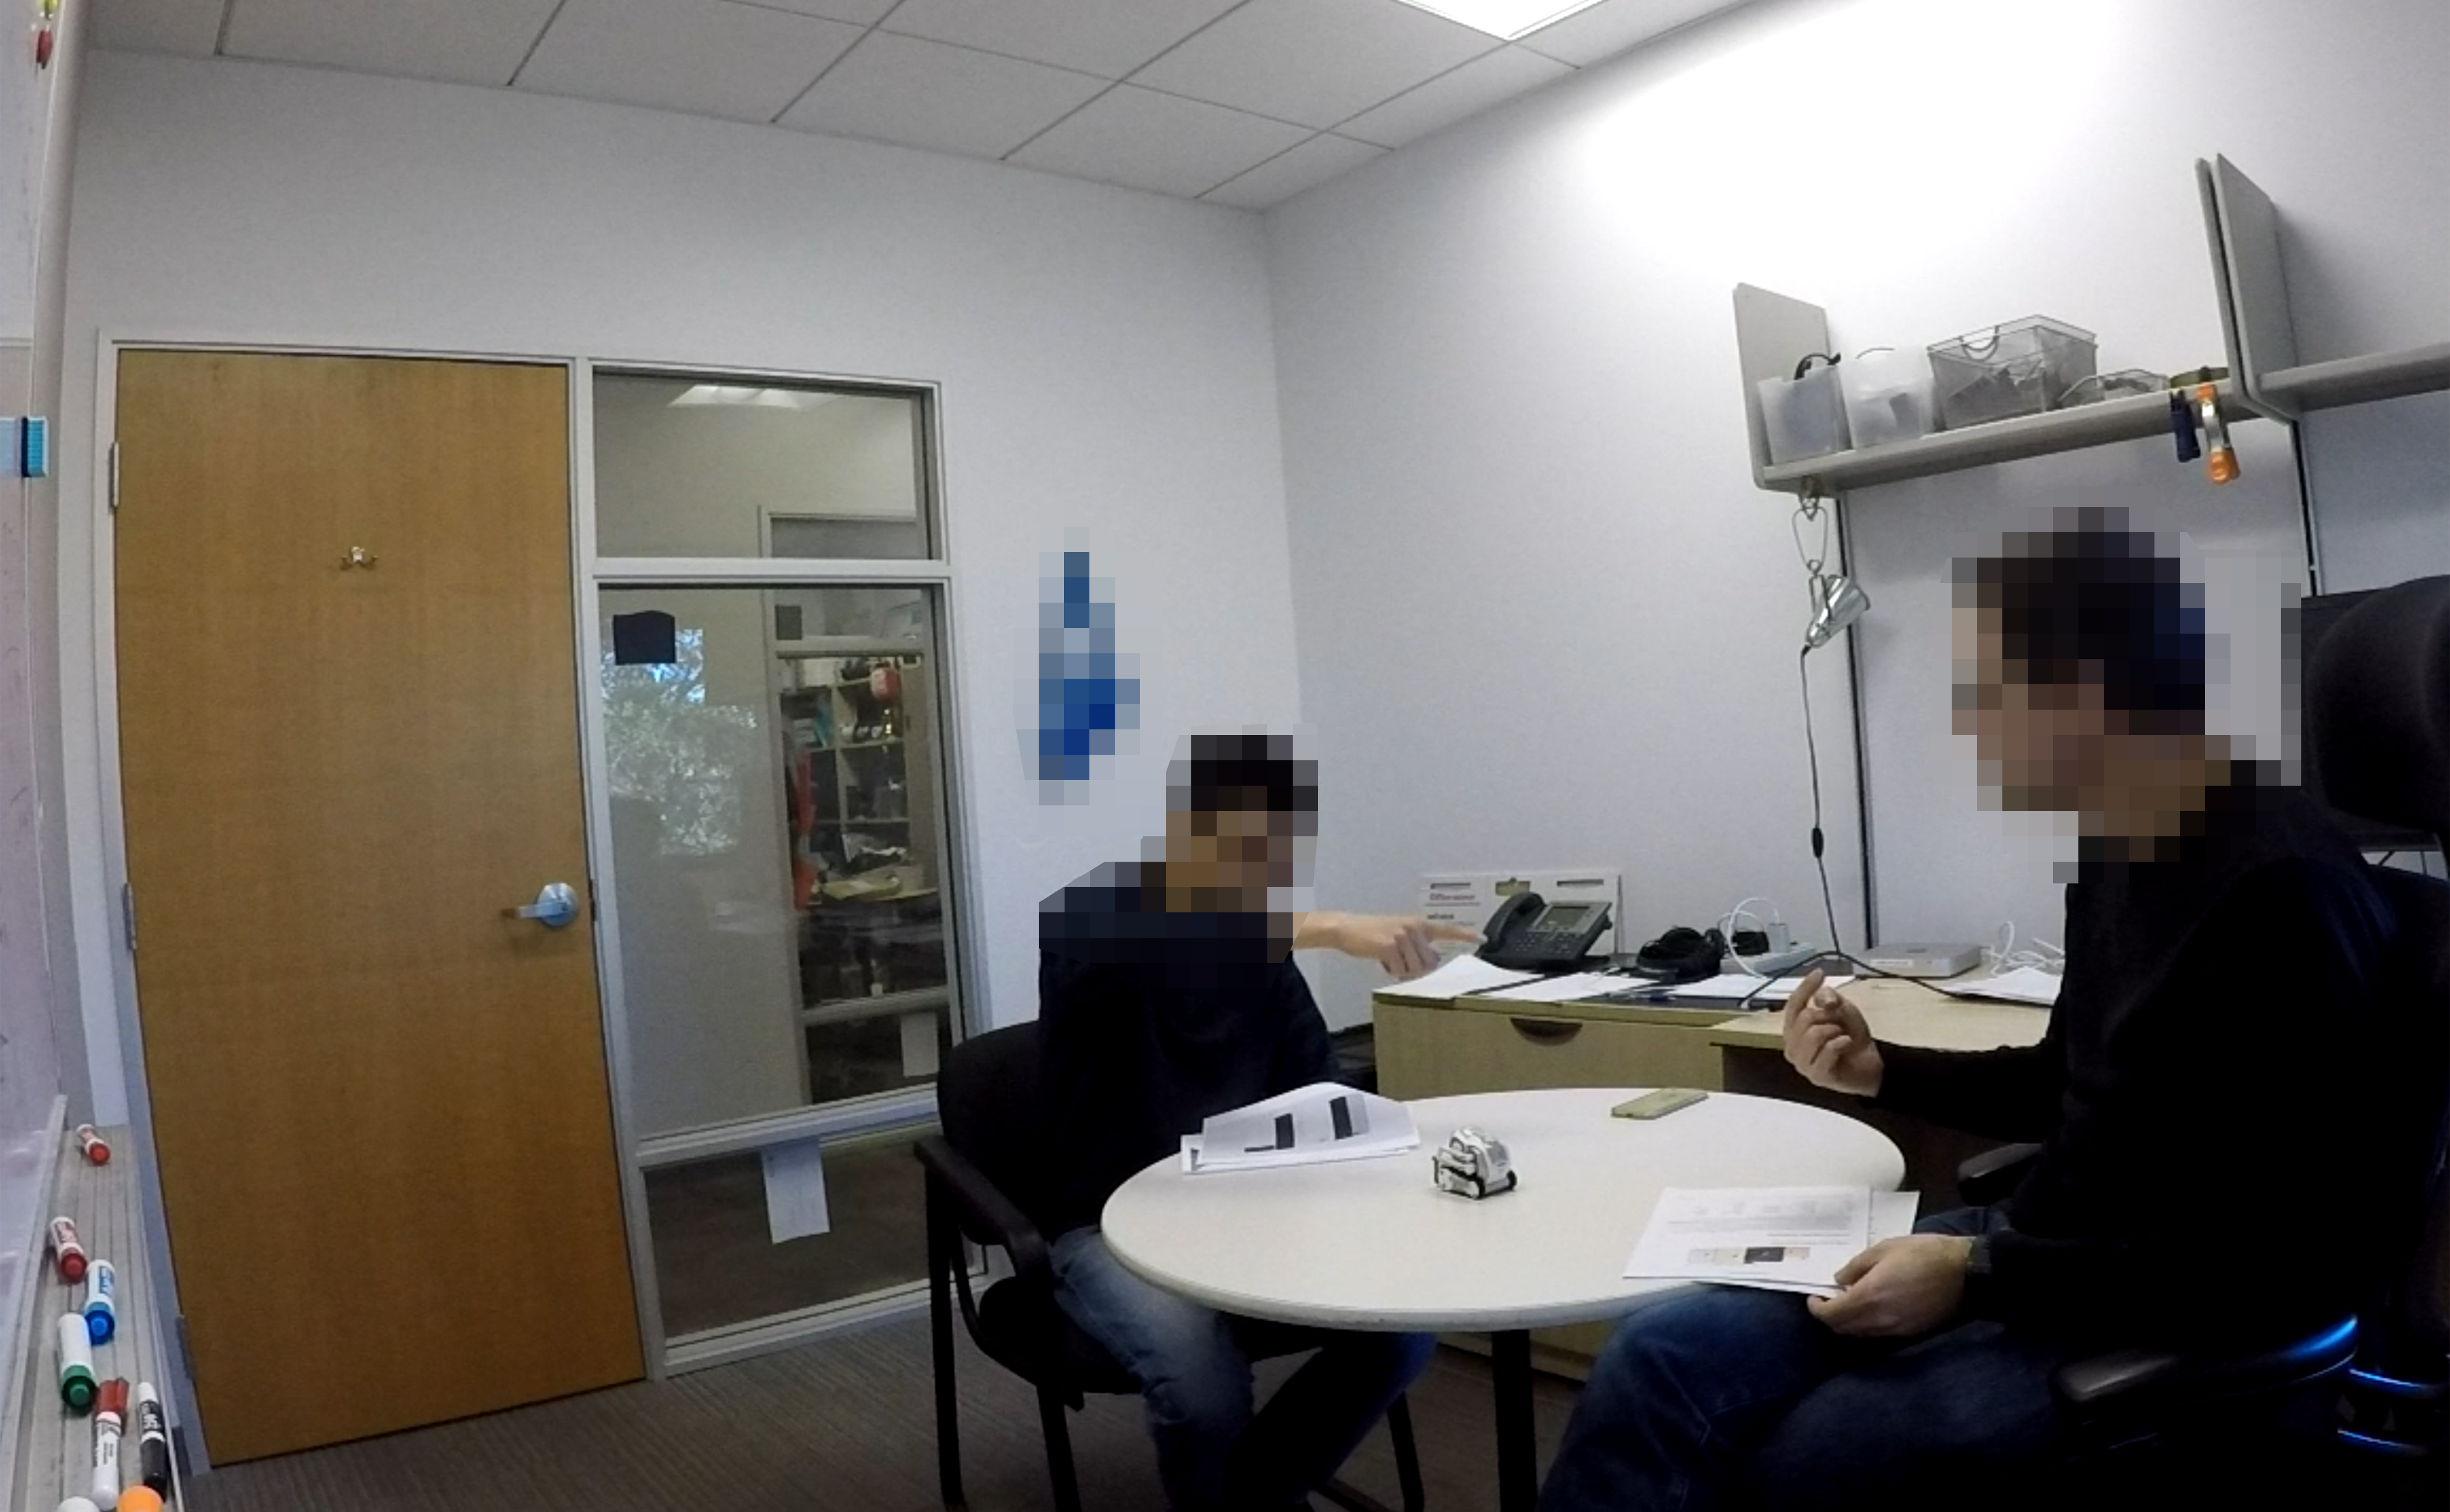
\includegraphics[trim={30cm 0 0
      0},clip,width=\columnwidth]{figures/gesturing}
  \caption{\label{fig:sub:gesture} Gesturing to the robot to move to P6.}
\vspace{2pc}
\end{subfigure}
\begin{subfigure}[b]{0.9\columnwidth}
  \centering 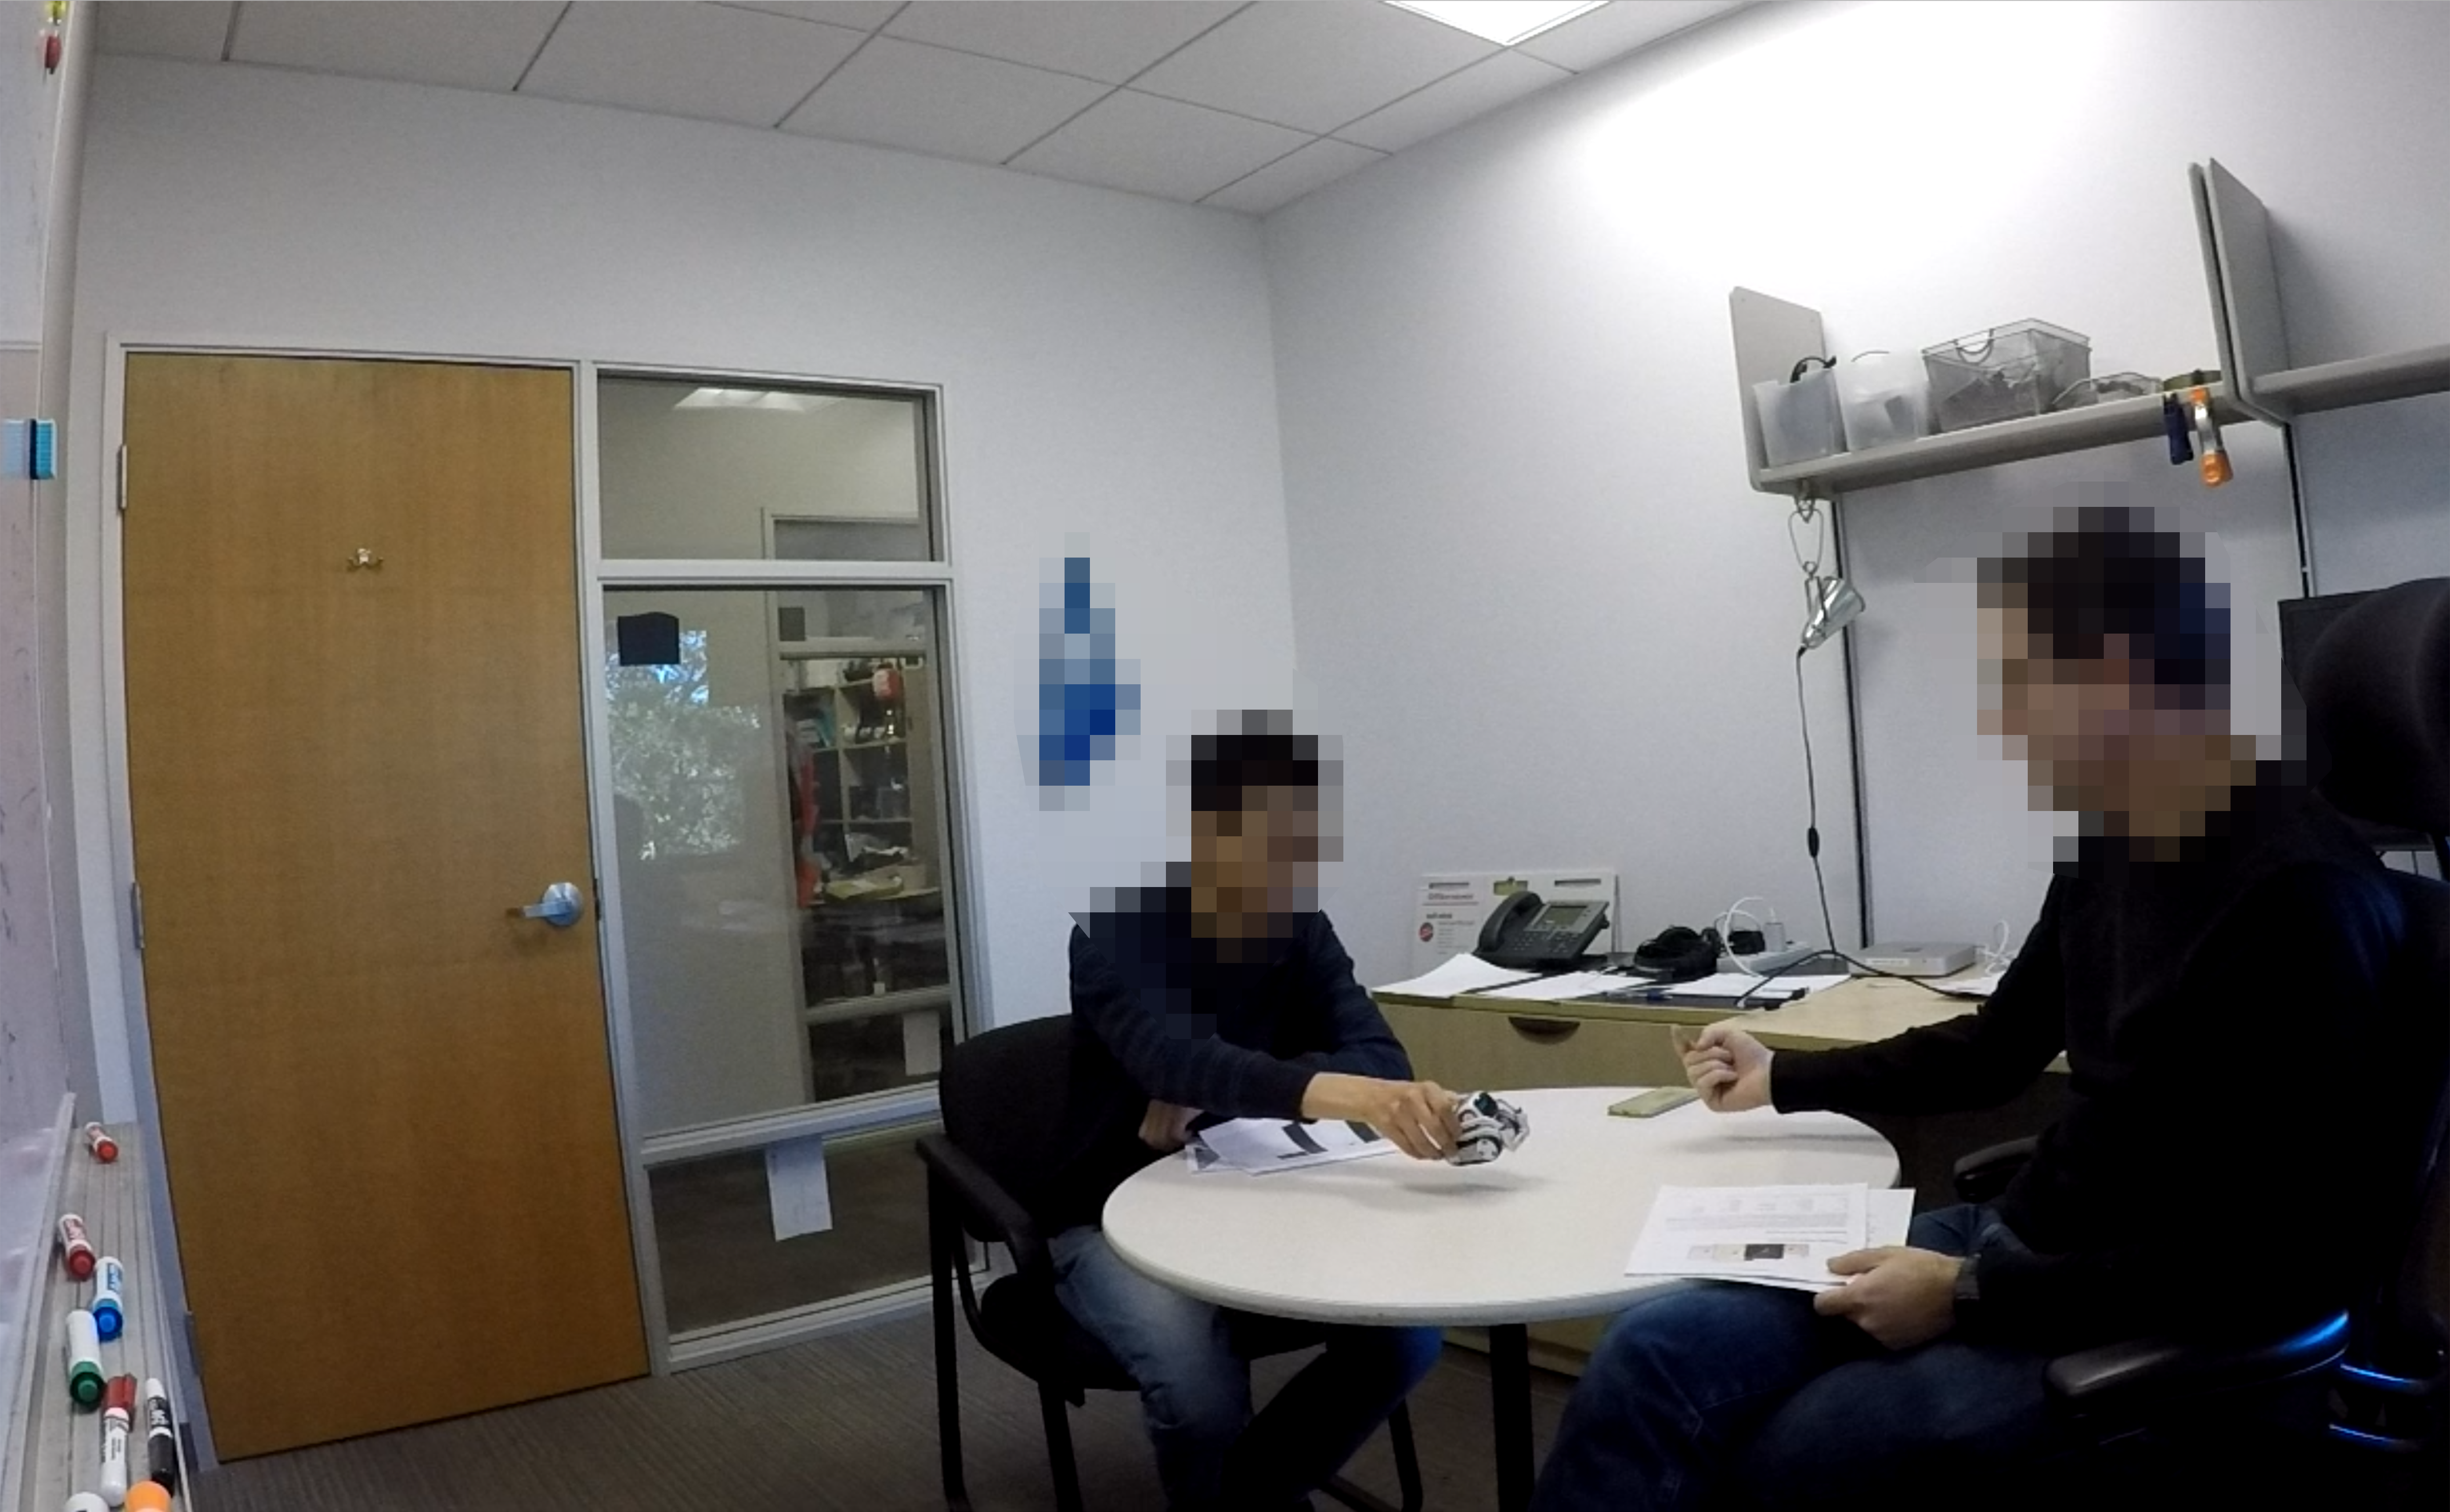
\includegraphics[trim={30cm 0 0
    0},clip,width=\columnwidth]{figures/gesturing-holding}
  \caption{\label{fig:sub:grab} P5, unhappy with the response time of
    the robot, picks it up and points it at P6.}
  \end{subfigure}
  \caption{\label{fig:gesture} P5 and P6 gesture to the robot
    mostly out of field. Eventually, P5 just picks up the robot and
    points it to P6. }
\end{figure}

\subsection{Gesture Driven Camera Robot}
One participant (P8) disagreed that the Gesture-Driven Camera Robot
was useful, while the rest agreed or strongly agreed. However, many
participants cited there was a bad recognition lag time on the robot
or that it was unclear to them what gestures they could actually use
to make it work.
\begin{quote}
``It seems gesture sensor is not so sensitive. And sometimes,
feel confused how to make the right gesture to the robot to work
well.'' (P7)
\end{quote}
Also, ``(I was) not sure how/what gestures can direct the robot.''
(P4). 

Of the participants who made some gestures in the robots field of
view, they still cited latency issues (likely partially due to the
WiFi streaming rate of the robot).  However, it was the case that most
participants would gesture outside of the field of view of the camera
and then slowly drop the gesture into the robots vision.  Once the
wizard could actually see the gesture from the robot's camera, it
would be enacted. Figure~\ref{fig:sub:gesture} shows two participants
from the GoPro in the room gesturing outside of the robot's vision.
Upon giving up, one participant just picked up the robot to turn it
manually to the other person (Figure~\ref{fig:sub:grab}). Four
participants physically moved the robot in this condition (P7, P8, P9,
and P10). One other participant asked if he was allowed to move the
robot, but only did so after the sessions were completed. In this
case, he thought ``why am I using my hands [to gesture] when I can
just do this?  (\textit{mimes picking up robot})'' (P8).

However, there were also some positive
points made about gesture control being natural ``It's like interacting
with real people, natural.'' (P5) and not distracting ``I dont have to
stop talking to give it instructions, nice.'' (P7).

\subsection{Voice controlled Camera Robot}
This condition had unanimous usefulness ratings: 4 with strongly agree
and 6 with agree.  We mimicked the interaction style of modern day
speech interfaces by having the ``hey robot'' trigger. During the
experiment, the robot (wizard) was rather flexible as many
participants said ``hello robot'' or ``hi robot.'' Many people enjoyed
this interaction.  ``It's interesting to talk to the robot, it's like
having a secretary.'' (P7), ``(It's) easy to change views, flexible in
conversation'' (P5), and
\begin{quote}
  ``I didn't need to learn a new control interface (Joystick). Seemed
  pretty responsive, not much delay, did basically what I expected!''
  (P8).
\end{quote}
Others cited difficulty: ``Takes effort to describe orientation
direction and how far to rotate.''~(P3) and ``If within arms reach,
easier to manually position or let remote person control it.'' (P6).

There were a few different interaction dynamics in this condition.  A
few participants (P3, P4, P5) gave relative-rotational instructions
like \textit{Turn $\{n\}\degree$ to the $\{d\}$}.  Others (P7, P8)
would say the degrees of rotation with a logical object (like
themselves) instead of clockwise or counterclockwise directive:
e.g. ``Turn 90\textdegree\ towards me''. Some participants (P9, P10)
would just say the trigger ``hey robot'' as the implicit \textit{Turn
  to me} command.  Finally some would give a logical object like
``turn to the whiteboard'' (P9) and others, noteably P4, stared with
hard coordinate directions ``Turn 70\textdegree\ to the left'' but
grew to say ``Robot get the whiteboard, the whiteboard'' by the end of
the 10 minute condition session.

\subsection{Issues with the Camera Robot}
There were some common issues with the Cozmo camera robot. First, many
participants mentioned it was noisy (P3, P4, P5, P8). While not
overwhelmingly loud, its motor driven tracks and head do make a
grinding noise that is uncommon in most video sessions (different than
the hum of a CPU or high-pitch sound of some electric devices). This
is more so recognized next to the silent 360\textdegree\ camera.  In
the context of recording, it introduced some difficulties: ``Made
obvious noise when moving so i had to talk over it.'' (P8)

There was some small frustration with not knowing the vocabulary of
commands, be them visual or audio, to give the robot (P3, P4, P6, P8)
but this was the part of the exercise of this elicitation study.  Also
a few participants (P6, P8) asked what was the point of having the
co-located presenters control the robot, as opposed to letting remote
person just have control of the robot in the first place?

%\subsection{Reactions to different modalities}
% Table~\ref{fig:likerts} presents the mean responses to the survey questions relating to the usefulness, awareness of, degree of control over, and distraction caused by the different conditions. While almost all conditions were rated above average in terms of usefulness, the 360-degree camera was rated lower than the robotic conditions in terms of agreement with the question "I knew what the camera was looking at."  ---PUT IN A QUOTE HERE ---


% \subsection{Observed behaviors from elicitation study: Gestures, voice, and task}
% \hl{Ayman will detail:Count how many interactions we saw.  Specify how many were
%   misunderstood, specify how many unique interactions were seen.
%   Break this down by gesture and voice.}

% \subsection{Gesture Control}
% \begin{itemize}
% \item Some gave gestures in the direct field of vision of the robot.
%   P1 P2
% \item Some gave gestures in the far peripheral vision of the robot. In
%   these cases, they would repeat the gesture until it was in frame
%   enough so the experimenter could take action. P3 P4
% \item P6 and P5 moved Cozmo while it was moving, causing it to overshoot
%   the whiteboard, they gestured for it go back a bit.
% \end{itemize}

% \subsection{Voice Control}
% \begin{itemize}
% \item Some said turn to [object] like ``Turn to me, or turn this way''
% \item P4 started saying ``Turn 180 Degrees to the Left'' but continued with ``Robot get the whiteboard, the whiteboard''
% \item Some said ``Turn 70 Degrees to the Right'' P3 P4 P5
% \end{itemize}

% \subsection{360}
% \begin{itemize}
% \item P6 held stuff to the 360\textdegree\ cam
% \item p3 p4 didnt hold stuff up assuming it would see it anyhow.
% \end{itemize}

% \subsection{AI}
% \begin{itemize}
% \item P6 still gestured to it in this state.  
% \end{itemize}

% \subsection{Other things}
% \begin{itemize}
% \item Some said they wanted to just move the robot. (P2 P4)
% \item P6 finally just moved the robot
% \item Some said they liked how they knew what the robot was looking at (P3)
% \item Some would just put the paper in the field of vision of the
%   robot instead of issuing another command. See Figure~\ref{fig:insertpage}.
% \end{itemize}

% \subsection{Reactions}
% \hl{Jenn can you add the quotes here?  For long quotes I do like
%   this:}
% \begin{quote}
%   ``I like the robot. Nullam eu ante vel est convallis dignissim.
%   Fusce suscipit, wisi nec facilisis facilisis, est dui fermentum
%   leo.'' (P2)
% \end{quote}
% Otherwise just quote inline like, ``No robots thanks'' (P3). 

\section{Discussion}
We investigated how people would interact with small smart camera
devices and how would they change the experience. Three advancements
motivate this work: more specialized devices are entering the consumer
market, modern deep AI is driving advancements in gesture and voice
interfaces, and finally, the growth of video communication (in
teleconferences, video calls, and livestreams). This study illustrates
not only what kind of commands people issue with smart cameras but
also how they manipulate the device (by physically moving it) and how
it can facilitate a better connection to the remote participant.

Overall, the participants found the cameras useful for presenting
visual information over a video stream. While the 360\textdegree\
camera was most often chosen as the most preferred when ranking the
four conditions, most of the conditions were thought to be useful.  We
did find several social and environmental observations which should be
considered for the future design of personal smart cameras.

\subsection{General Observations}
First, we note that most of the participants asked for feedback from
the device.  No feedback was given from the Cozmo robot despite it
having colored lights, text-to-speech, and can nod to say yes or shake
in disagreement. This was to keep it close to the 360\textdegree\
camera which had no feedback capabilities.  Further, many participants
asked for a preview window of the devices and previous work has shown
its value in media spaces~\cite{Mok:2017:CPP:3064663.3064722} and
livestream chats~\cite{Shamma:2009:SOC:1556460.1556486}. This was not
in the study design as we wanted to focus on the interaction with the
device and not self positioning in the preview frame.

In the cases where the robot had a gesture or voice control, many
participants initially paused wondering what to gesture or say.
Typically, when one participant would invent a command, the other
would repeat a similar command.  This dissipated over the course of
each session as the participants started inventing newer commands, but
was something to note.  While most all the participants would
generally control the camera for themselves, a few participants would
give a command for the other participant.  In one case, P5 gestured to
move the camera to P6 (Figure~\ref{fig:gesture}).  In another, P10
generally just moved the camera by hand for P9.

\subsection{Awareness}
By withdrawing feedback, our experiment highlighted the importance of
feedback delivery to the participants, especially with gesture
control. Adding audio (tones or voice) output or visual displays
showing what the robot is capturing could help alleviate these issues
but also run the risk of distracting the video with sound or another
screen in the frame. A screen would need to be on the camera-device as
not to have someone look one direction to fix the camera in the other
direction.

When it comes to voice commands, some participants directly addressed
the robot by naming objects (e.g.\ ``get the whiteboard'', ``back to
me'').  The robot needs to develop an awareness of its surroundings,
remember its surroundings, or slowly build and remember the context to
be fully operational as soon as possible. In particular, the AI will
need to recognize common objects and their location given the context
and task (meeting room, cooking show, family video call, etc.).

Overall, having a camera that knows where to look was seen as having
value if one knows where it is looking.  And while the 360\textdegree\
camera's silent omnicapture was preferred, the robot having a focus
and attention brought it into the meeting as more of a
participant. Conversely, the design of how a 360\textdegree\ camera
could indicate its focus point merits exploration. In either case,
there is a trade-off between awareness and interruption that must be
taken into consideration.

\subsection{Camera Position}
Most participants held papers up in front of the camera, both with the
robot and the 360\textdegree\ camera. In some cases, they were holding
the paper and still pointed at figures or paragraphs. If the
360\textdegree\ camera had instead been mounted above the table
looking down, the users might have felt no need to hold their paper
sheets. However, the aforementioned benefit of the robot on the desk
makes it feel like more of a tool for engagement. This prompted
several participants to pick it up and move it. A very portable and
light-weight robot certainly encourages that kind of interaction.  The
physical design of a desk robot should have several view points.
While many media spaces have conversations that are gaze-forward (to
another) or gaze-down (to an
object)~\cite{Mok:2017:CPP:3064663.3064722}, the design of such a desk
camera robot should support both and possibly correct perspective.
This is something that is lacking in common cameras on laptops and
tablets and even more modern devices like the Meeting Owl.

\subsection{Laptops and Other Screens}
While this experiment used papers and a whiteboard, many meetings and
video sessions involve sharing screens from laptops, tablets, and
smart phones. Indeed, half of our participants (P4, P7, P8, P9, P10)
stated they would like the Cozmo to look at a laptop or device
screen. This could be treated as any other media object or document
where the participants turn their laptops toward the camera, like they
did holding paper sheets.  However, a small portable focused device
could sit to the side of a user at the table's edge or even be
positioned between a user and the device. Here, a device like a Cozmo
could track a screen or hand-held device and, as our study elicited,
keep users informed on what the camera is capturing.  By contrast,
placing a 360\textdegree\ camera between a device and a person could
lead to some potentially unflattering vantage points for the
participants. Even if the device has the AI smarts not to show faces
from under ones nose, for example, users still might wonder if that is
what it is capturing.

\section{Conclusions}
In this article, we describe insights from a Wizard-of-Oz elicitation
study to inform the design of AI-powered interactions for the future
of consumer camera support for video calling and livestreaming. While
the silent, still 360\textdegree\ camera was preferred by the
participants, it carried the understanding that it was auto-panning
and cropping by itself; with that, participants still wondered where
it was looking. Cameras that can ``look'' in a direction, such as the
Cozmo, provide such an indication of where it is pointed but introduce
some distractions. Coupled with an auto-AI engine, participants
considered the robot more of a meeting participant than the
360\textdegree\ camera---in effect, the shared consumer device felt
more like a personal device facilitating conversation.  However, most
consumer devices are not well designed for these interactions and we
have illustrated both insights for the physical design and interaction
techniques required for next generation video cameras for streaming.

%\section{Acknowledgments}
%Withheld for review.

\balance%

\bibliographystyle{SIGCHI-Reference-Format}
\bibliography{hci}

\end{document}

%%% Local Variables:
%%% mode: latex
%%% TeX-master: t
%%% End:
